%!TEX root = presentazioneNBD.tex

\setlength{\parskip}{\baselineskip} 
\section{Definitions and literature}
\begin{frame}[t]
\frametitle{Definitions and literature}
\begin{block}{What is going to be explained?}
	\begin{itemize}
		\item Thesis
		\item Single Commodity Flow Problems
		\item Multicommodity Flow Problems
		\item Prior work on max-flows and min-cuts for multicommodity flow problems
		\item Max-flow min-cut results
		\item Applications to Approximation Algorithms
		\item Subsequent Work
	 \end{itemize} 
\end{block}
\end{frame}

\begin{frame}
%\subsection{Thesis}
\frametitle{Thesis}
Relationship between maximum flow and minimum cut in multicommodity flow problem

Previous Literature:\\
Ford and Fulkerson [1956]
max-flow and min-cut always equal in 1-commodity flow problems
\end{frame}


\begin{frame}
%\subsection{Single Commodity Flow Problems}
\frametitle{Single Commodity Flow Problems}
1-commodity flow problems
\begin{itemize}
	\item $n$ nodes $V$
	\item $m$ edges $E$
	\item non negative capacity $C(e)$ for each $e \in E$. 
	% Maximum amount of flow that can pass through the edge (if not specified, we assume that the edges are undirected)
	\item nodes designation: 
	\begin{itemize}
		\item \textit{source} $s$
		\item \textit{sink} $t$
	\end{itemize}
\end{itemize}
\end{frame}


\begin{frame}
\frametitle{Single Commodity Flow Problems}
\textit{Objective:}\\
to route as much flow as possible from the source to the sink without violating the capacity of any edge.

\textit{max-flow:}\\
maximum amount of flow that can be routed.

\textit{min-cut:}\\
minimum amount of capacity that needs to be removed from the network in order to disconnect the source from the sink. Formally:
$$\min_{ \{ U \subset V | s \in U, t \in \bar{U} \} } \sum_{e \in \langle U, \bar{U} \rangle } C(e)$$
%U is any subset of V that contains the source but not the sink
%$\bar{U} = V - U$ the set of nodes not in U
%$\langle U, \bar{U} \rangle$  set of edges that link a node in U to a node in $\bar{U}$ 
\end{frame}

\begin{frame}
\frametitle{Single Commodity Flow Problems}
\textit{cut of the network:}\\
set of edges from any set $U$ to $\bar{U}$ since the removal of those edges separates $U$ from the rest of the network.

\textit{min-cut 1-commodity flow problem is always an upper bound on the max-flow. Why?}\\
For any $U \subseteq V$ that contains the source but not the sink, all flow from $s$ to $t$ must be routed through edges in  $\langle U, \bar{U} \rangle $. Hence, the total flow is limited by the capacity in the min-cut.
\end{frame}


\begin{frame}[c]
\frametitle{Single Commodity Flow Problems}
	\begin{figure}
		\centering
		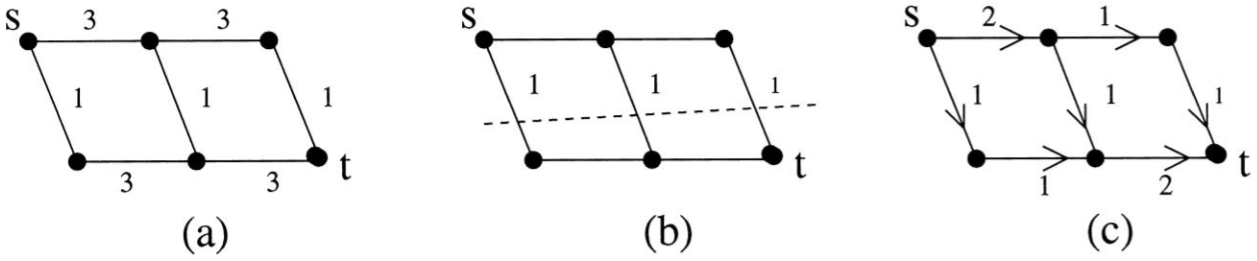
\includegraphics[width=\textwidth]{figs/1-commodity_flow_problem.png}
		\caption{Solution to a 1-commodity flow problem}
		\end{figure}
\end{frame}


\begin{frame}
%\subsection{Multicommodity Flow Problems}
\frametitle{Multicommodity Flow Problems}
\begin{center}
\textit {k $ \ge 1$}\\
\end{center}

$k$ number of commodities, each with source $s_i$, sink $t_i$ and demand $D_i$

\textit{Objective:}\\
simultaneously route $D_i$ units of commodity $i$ from $s_i$ to $t_i$ for each $i$ so that the total amount of all commodities passing through any edge is no greater than its capacity.
%undirected edges the sum of the flow in both directions cannot exceed the capacity of the edge.
%useful to maximize the amount of flow that can be routed for each commodity.
\end{frame}


\begin{frame}
\frametitle{Multicommodity Flow Problems}
\textit{concurrent max-flow:}\\
maximize a common fraction $f$ of each commodity that is routed. In other words the maximum value of $f$ such that $fD_i$ units of commodity $i$ can be simultaneously routed for each $i$ without violating any capacity constraints.

\textit{fairness property:}\\
ensures that proportionally more of one commodity will not be routed at the expense of another.

\textit{min-cut (a.k.a sparset cut $\mathscr{S}$):}\\
the minimum over all cuts of the ratio of the capacity of the cut to the demand of the cut.
\end{frame}

\begin{frame}
\frametitle{Multicommodity Flow Problems}
$$ \mathscr{S} = \underset{U \subseteq V }{min} \frac{C(U,\bar{U})}{D(U,\bar{U})}, $$
where 
$$ C(U,\bar{U}) = \sum_{e \in \langle U, \bar{U} \rangle} C(e) $$
is the sum of capacities of the edges linking $U$ to $\bar{U}$ and 
$$ D(U,\bar{U}) = \sum_{ \{ i | s_i \in U \land t_i \in \bar{U}\quad or \quad t_i \in U \land s_i \in \bar{U} \} } D_i $$
is the sum of the demands whose source and sink are on opposite sides of the cut that separates $U$ from $\bar{U}$
\end{frame}

\begin{frame}[c]
\frametitle{Multicommodity Flow Problems}
	\begin{figure}
		\centering
		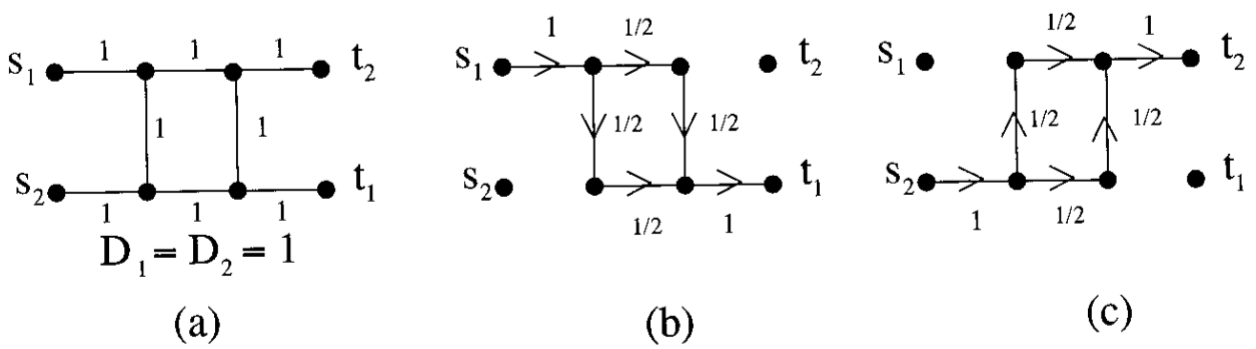
\includegraphics[width=\textwidth]{figs/2-commodity_flow_problem.png}
		\caption{Solution to a 2-commodity flow problem}
	\end{figure}
\end{frame}


\begin{frame}
\frametitle{Multicommodity Flow Problems}
Check that the \textit{max-flow} is always upper bounded by the \textit{min-cut} for any multicommodity flow problem. Let $i_1,i_2,i_3,\dots,i_r$ denote the commodities  whose source and sink are separated by some cut $\langle U, \bar{U} \rangle$
$$	\sum_{j=1}^{r} fD_{i_{j}} \le C(U, \bar{U})	$$
Since
$$	\sum_{j=1}^{r} D_{i_{j}} = D(U, \bar{U})	$$
this means that
$$	f \le \frac{C(U, \bar{U})}{D(U, \bar{U})}	$$
%the max flow is upper bounded by the min-cut
\end{frame}


\begin{frame}
%\subsection{Prior work on max-flows and min-cuts for multicommodity flow problems}
\frametitle{Prior work on max-flows and min-cuts for multicommodity flow problems}
Schrijver [1990]\\
If the graph formed by the set of demands does not contain either three disjoint edges or a triangle and a disjoint edge\\
\quad ---> \quad \textit{max-flow and min-cut are equal}

Example: when there is a commodity for every pair of nodes and all demands are equal, the max-flow and min-cut are equal provided that the dual of the flow problem satisfies a certain cut condition.

\textit{general networks}\\  
The max-flow is within a factor of $k$ of the min-cut since each commodity can be optimized separately using 1/k of the capacity of each edge.
\end{frame}

\begin{frame}
\frametitle{Prior work on max-flows and min-cuts for multicommodity flow problems}
	\begin{figure}
 		\centering
    		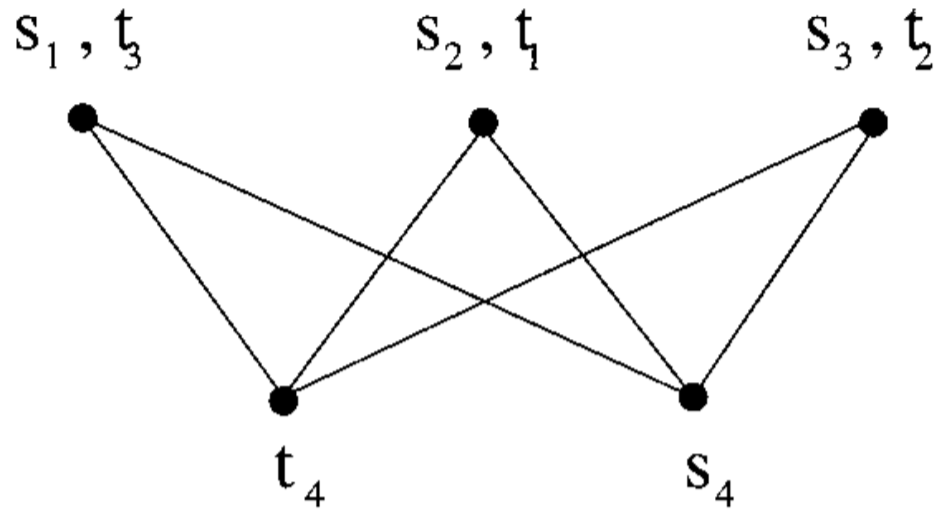
\includegraphics[width=0.5\textwidth]{figs/3-Okamura_Seymour.png}
		\caption{Okamura-Seymour [1981] with max-flow=3/4 and min-cut=1}
	\end{figure}
\end{frame}


\begin{frame}
%\subsection{Max-flow min-cut results}
\frametitle{Max-flow min-cut results}
	 \textit{UMFP (Uniform Multicommodity Flow Problem)}\\
	 In this kind of flow problem there is a commodity for every pair of nodes and the demand for every commodity is the same. WLOG the demand for every commodity is set to one.
	 %Without Loss Of Generality
\end{frame}

\begin{frame}
\frametitle{Max-flow min-cut results}
\begin{block}{What is going to be proved?}
	\begin{itemize}
		\item An approximate max-flow min-cut theorem for uniform multicommodity flow problems. 
		The max flow is within a $\Theta (\texttt{log} n)$-factor of the min-cut. 
		\item The previous bound is tight in the sense that there exist uniform flow problems for which the max-flow is precisely a factor of $\Theta(\texttt{log}n)$ smaller than the min-cut for any $n$.
		% Also we show that this bound is tight in the sense that there exist uniform flow problems for which the max-flow is precisely a factor of $\Theta(\texttt{log}n)$ smaller than the min-cut for any $n$.
	 \end{itemize} 
\end{block}
\end{frame}


\begin{frame}
\frametitle{Max-flow min-cut results}
What is $\Theta$?\\
For a given function $g(n)$, we denote by $\Theta (g(n))$ the set of functions
\begin{equation*}	
	\begin{split}
		\Theta(g(n)) = \{ f(n) : & \text{ $\exists \quad c_1, c_2 > 0$ and $n_0$ such that} \\
						 & 0 \le c_1 g(n) \le f(n) \le c_2 g(n) \quad \forall n \ge n_0 \}
	\end {split}
\end{equation*}
\end{frame}

\begin{frame}
\frametitle{Max-flow min-cut results}
	\begin{figure}
 		\centering
    		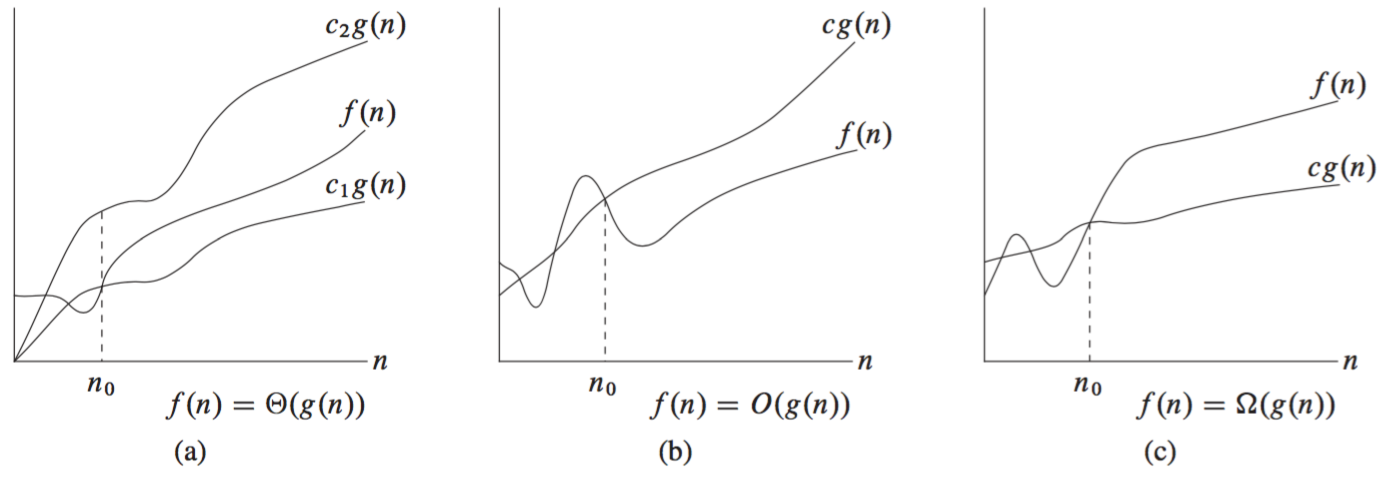
\includegraphics[width=\textwidth]{figs/4-Asymptotic_notation.png}
		\caption{Graphic examples of the $\Theta$, $O$, and $\Omega$  notations. (a) $\Theta$-notation bounds a function to within constant factors. (b) $O$-notation gives an upper bound for a function to within a constant factor. (c) $\Omega$-notation gives a lower bound for a function to within a constant factor.}
%Graphic examples of the $\Theta$, $O$, and $\Omega$  notations. In each part, the value of $n_0$ shown is the minimum possible value; any greater value would also work. (a) $\Theta$-notation bounds a function to within constant factors. We write $f(n) = \Theta (g(n))$ if there exist positive constants $n_0$, $c_1$, and $c_2$ such that at and to the right of $n_0$, the value of $f(n)$ always lies between $c_1 g(n)$ and $c_2 g(n)$ inclusive. (b) $O$-notation gives an upper bound for a function to within a constant factor. We write $f(n) = O(g(n))$ if there are positive constants $n_0$ and $c$ such that at and to the right of $n_0$, the value of $f(n)$ always lies on or below $cg(n)$. (c) $\Omega$-notation gives a lower bound for a function to within a constant factor. We write $f(n) = \Omega (g(n))$ if there are positive constants $n_0$ and $c$ such that at and to the right of $n_0$, the value of $f(n)$ always lies on or above $cg(n)$.
	\end{figure}
\end{frame}



\begin{frame}
%\subsection{Applications to Approximation Algorithms}
\frametitle{Applications to Approximation Algorithms}
In a UMFP we have:\\
\textit{Demand} across a cut $\langle U, \bar{U} \rangle$ 
%is the product of the number of nodes in $U$ and the number of nodes in $\bar{U}$
$$D(U,\bar{U}) = |U||\bar{U}|$$
\textit{Min-cut} of uniform flow problem is
$$ \mathscr{S} = \underset{U \subseteq V}{min} \frac{C(U,\bar{U})}{ |U||\bar{U}|}$$
where $C(U,\bar{U}) = \sum_{e \in \langle U, \bar{U} \rangle } C(e)$.\\
In the case when all capacities are 1, the min-cut is simply
$$ \mathscr{S} = \underset{U \subseteq V}{min} \frac{| \langle U,\bar{U}\rangle |}{ |U||\bar{U}|}$$
\end{frame}

\begin{frame}
\frametitle{Applications to Approximation Algorithms}
\textit{min-cut} is a good measure of the number of edges that need to be removed in order to partition the underlying network into pieces of various sizes.

\textit{Consequence:} able to use our algorithm for finding an approximate min-cut to design the first nontrivial polynomial-time approximation algorithms for several important NP-hard graph partitioning problems.
\end{frame}


\begin{frame}
%\subsection{Subsequent Work}
\frametitle{Subsequent Work}
More literature and results of this paper was published at the first time in an extended abstract of Leighton and Rao [1988].\\

Subsequent work:
\begin{itemize}
	\item Klein et al. [1995] the max-flow is always within an $O(\texttt{log} C \texttt{log} D)$ factor of the min-cut for undirected multicommodity flow problems.
	\item Tragoudas [1990], Plotkin and Tardos [1993] and Garg et al. [1996] have improved the previous bound to $O(\texttt{log}^2 k)$
	\item Linial  et al. [1995] and Aumann and Rabani [1998] established an existentially tight gap of $\Theta(\texttt{log} k)$ with the use of Bourgain's technique with embed spaces on graphs into geometric spaces.
\end{itemize}
\end{frame}	

\begin{frame}
\frametitle{Subsequent Work}
\begin{itemize}	
	\item Garg  et al. [1996] established an $O(\texttt{log} k)$  max-flow min-cut theorem for arbitrary (undirected) multicommodity flow problems where the sum of the flows is maximized. 
	\item Klein et al. [1993] discovered a $\Theta(1)$ max-flow min-cut theorem for uniform multicommodity flow problems in undirected planar graphs and graphs with small excluded minors.
	\item Klein et al. [1997] and Even et al. [1998] $O(\texttt{log}^3 k)$ max-flow min-cut theorem for multicommodity flow problems in directed networks for which the demand from any node u to any node v is equal to the demand from v to u. 
\end{itemize}
\end{frame}




